%!TEX root = ../thesis.tex
% створюємо розділ
\chapter{Розробка власного смарт-контракту}
\label{chap:theory}

Для розробки смарт-контракту потрібно визначитись із:
\begin{itemize}
    \item мовою програмування смарт-контрактів,
    \item середовищем розробки смарт-контрактів,
    \item інструментами тестування та розгортання смарт-контрактів.
\end{itemize}

\section{Мова програмування смарт-контрактів}

Для написання власного смарт-контракту в тестовій мережі Sepolia ми обрали мовою програмування Solidity. 

    \begin{figure}[ht]
        \centering
        
\includegraphics[scale=0.5]{IMAGES/solidity-logo.png}
        \caption{Лого мови програмування Solidity.}
        \label{fig_sudak}
    \end{figure}

Це обумовлено тим, що Solidity є найпопулярнішою мовою для розробки смарт-контрактів на платформі Ethereum, забезпечуючи широку підтримку інструментів та ресурсів для розробників. Крім того, вона має зручний синтаксис, схожий на JavaScript, що спрощує навчання та написання коду. Solidity забезпечує високу безпеку та ефективність, що є критично важливим для створення надійних та захищених смарт-контрактів.

Solidity також відзначається своєю сумісністю з різними тестовими мережами, такими як Sepolia, що дозволяє розробникам тестувати свої контракти в безпечному середовищі перед їх впровадженням у основну мережу. Це надає можливість виявляти та виправляти помилки на ранніх етапах розробки, що значно підвищує якість кінцевого продукту. Вибір Solidity також забезпечує легку інтеграцію з іншими інструментами екосистеми Ethereum, такими як Truffle та Remix, що прискорює процес розробки та розгортання смарт-контрактів.

\section{Середовище розробки смарт-контрактів}

Для написання власного смарт-контракту в тестовій мережі Sepolia ми використаємо середовище розробки Visual Studio Code (VSC). Visual Studio Code є одним із найпопулярніших редакторів коду, завдяки своїй безкоштовності, відкритому вихідному коду та широкому набору функцій, що робить його ідеальним вибором для розробників. 

    \begin{figure}[ht]
        \centering
        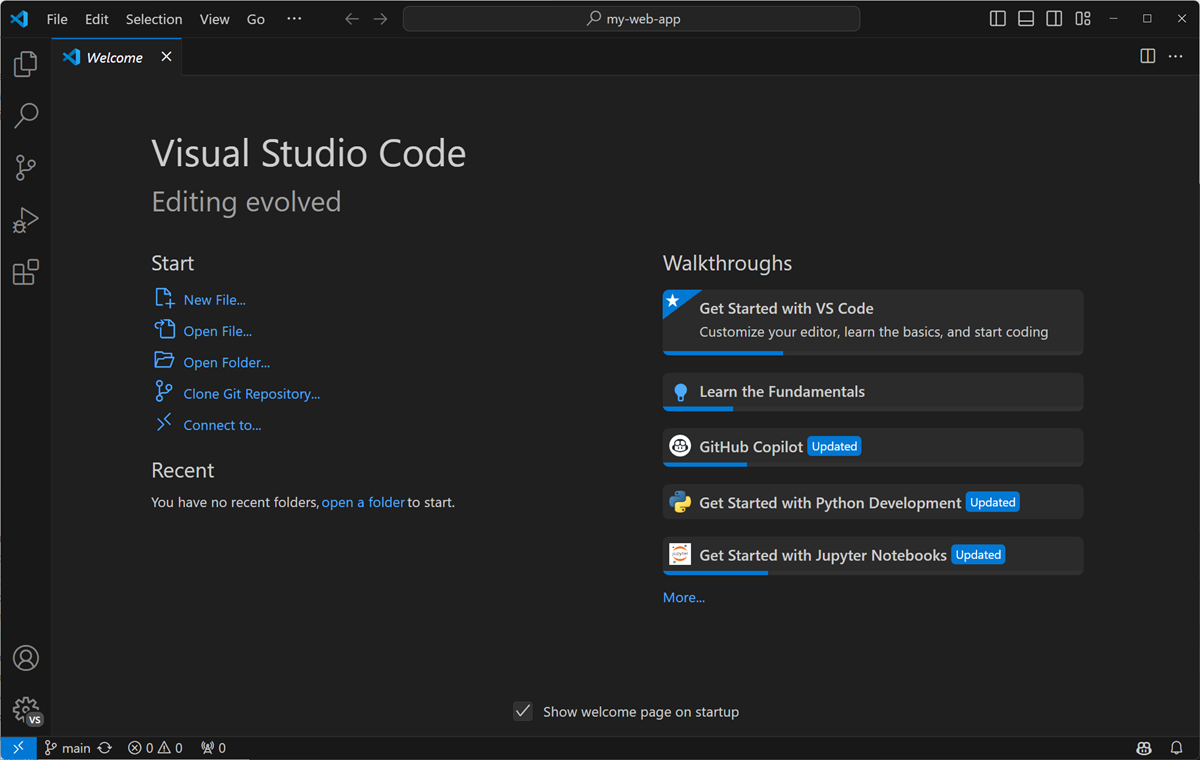
\includegraphics[scale=0.6]{IMAGES/vsc-page.png}
        \caption{Сторінка середовища Visual Studio Code.}
        \label{fig_sudak}
    \end{figure}

Додатково встановимо плагін Solidity, який додає підтримку синтаксису, автозаповнення, інтеграцію з компіляторами та інструментами для тестування смарт-контрактів, що значно спрощує процес розробки. 

Для цього в Visual Studio Code потрібно знайти та перейти до розділу розширення (англ. Extensions) в боковій панелі зліва, після -- в пошуку вписати Solidity, обрати зі списку наступне розширення та встановити його:

    \begin{figure}[ht]
        \centering
        
\includegraphics[scale=0.6]{IMAGES/solidity-extension-vsc.png}
        \caption{Розширення Solidity в маркетплейсі Visual Studio Code.}
        \label{fig_vsc}
    \end{figure}

    Після цього сторінка даного плагіну в маркетплейсі Visual Studio Code (VSC) буде виглядати наступним чином:

    \begin{figure}[ht]
        \centering
        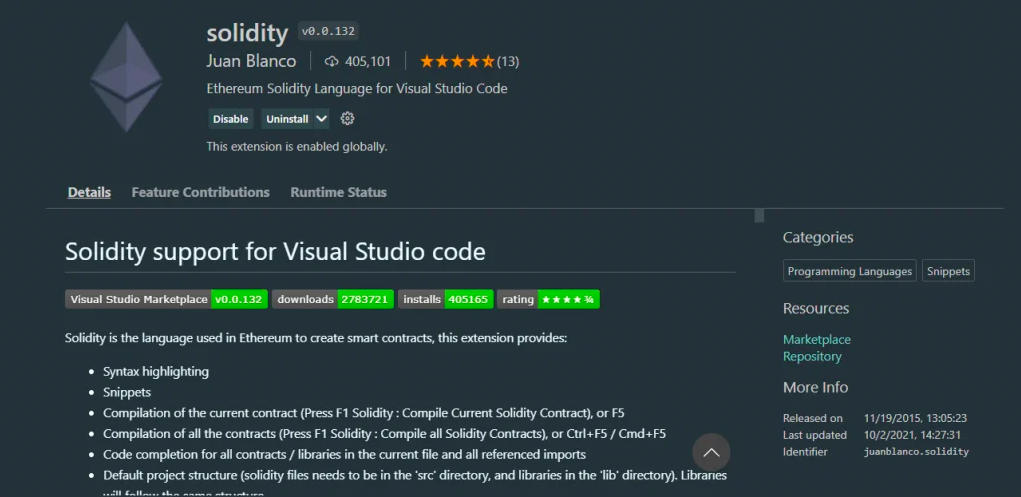
\includegraphics[scale=0.45]{IMAGES/solidity-extension-vsc1.png}
        \caption{Встановлення плагіну Solidity в середовищі VSC.}
        \label{fig_vsc}
    \end{figure}

Крім того, Visual Studio Code підтримує численні розширення та налаштування, що дозволяє розробникам адаптувати середовище під свої потреби, підвищуючи продуктивність та комфорт роботи. Завдяки цим перевагам, ми можемо ефективно розробляти, тестувати та налагоджувати наші смарт-контракти в Sepolia, забезпечуючи їх високу якість та надійність.

\section{Інструменти тестування та розгортання смарт-контрактів}

Для тестування та розгортання власного смарт-контракту в тестовій мережі Sepolia ми використаємо інструмент Hardhat. 

    \begin{figure}[ht]
        \centering
        
\includegraphics[scale=0.2]{IMAGES/hardhat-logo.png}
        \caption{Середовище розробки та тестування Hardhat.}
        \label{fig_vsc}
    \end{figure}

Hardhat є потужним фреймворком для розробки на Ethereum, що пропонує широкий спектр можливостей для компіляції, налагодження, тестування та розгортання смарт-контрактів. Однією з головних переваг Hardhat є його гнучкість та розширюваність, що дозволяє інтегрувати різні плагіни та інструменти для оптимізації процесу розробки. 

Крім того, Hardhat має вбудовану локальну блокчейн-мережу, яка дозволяє швидко тестувати контракти без необхідності використовувати зовнішні тестові мережі. Завдяки своїй потужній системі налагодження, Hardhat дозволяє легко відстежувати та виправляти помилки в коді, що значно підвищує якість кінцевого продукту. 

Використання Hardhat для тестування та розгортання смарт-контрактів в Sepolia забезпечує надійний і ефективний процес розробки, що дозволяє створювати безпечні та функціональні децентралізовані додатки.

\section{Написання смарт-контракту}

Розпочнемо написання смарт-контракту власного токену.

\vspace{0.5cm}
\textbf{Основні характеристики, яким має відповідати наш токен:}
\begin{enumerate}
    \item Початкова поставка токенів (відправлення власнику) = 70 000 000;\\
    \textit{Коли смарт-контракт токена буде створений, 70 000 000 токенів будуть автоматично відправлені власнику (наприклад, адресі, яка розгортає смарт-контракт). Це називається початковою (або первісною) поставкою токенів.}
    \item Максимальна пропозиція (обмежена) = 100 000 000;\\
    \textit{Встановлення верхньої межі загальної кількості токенів, які можуть коли-небудь існувати. Це означає, що незалежно від обставин, більше ніж 100 000 000 токенів не можуть бути створені. Це допомагає запобігти інфляції та забезпечує контрольоване розповсюдження токенів.}
    \item Токен повинен мати функціонал для спалювання токенів;\\
    \textit{Спалювання токенів зазвичай використовується для зменшення загальної пропозиції, що може підвищити вартість решти токенів. У Solidity це реалізується за допомогою функції \texttt{burn}.}
    \item Механізм винагороди майнерів за підтвердження нових блоків у блокчейні (\texttt{blockReward}, \texttt{\_beforeTokenTransfer}, \texttt{\_mintMinerReward}).
\end{enumerate}

\vspace{0.5cm}
Для надійної та безпечної реалізації багато розробників обирають стандарт токенів ERC20 від OpenZeppelin. Тому ми будемо використовувати контракт OpenZeppelin ERC-20 для створення нашого токена. З OpenZeppelin нам не потрібно писати весь інтерфейс ERC-20. Замість цього ми можемо імпортувати бібліотечний контракт і використовувати його функції.

\newpage
\textbf{Маємо наступнй функціонал нашого смарт-контракту:}

\begin{enumerate}

    \item Конструктор смарт-контракту \texttt{constructor}, який забезпечує початкове налаштування контракту для подальшого використання та необхідні початкові параметри для функціонування токену:

    \begin{figure}[ht]
        \centering
        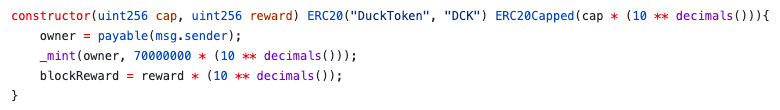
\includegraphics[scale=0.6]{IMAGES/code1.png}
        \label{fig_vsc}
    \end{figure}
    
    \textit{Він викликає конструктор базового контракту ERC20Capped з переданим значенням cap (обмеження на максимальну кількість токенів, що можуть існувати) та конструктор базового контракту ERC20, який ініціалізує токен з ім'ям «DuckToken» та символом «DCK». Передає власника контракту, встановлює початкову поставку токенів і встановлює винагороду за блок (reward).}
    
    \item Внутрішня функція \texttt{\_update}, яка оновлює стан токену після кожної операції передачі токенів.
    
    \begin{figure}[ht]
        \centering
        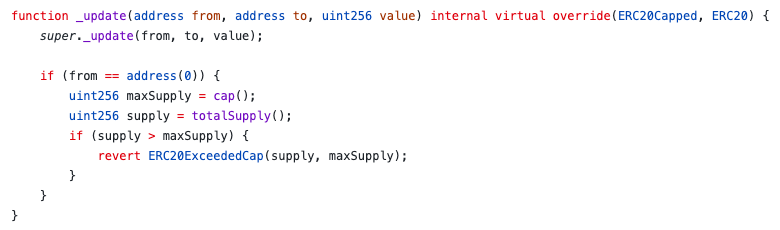
\includegraphics[scale=0.6]{IMAGES/code2.png}
        \label{fig_vsc}
    \end{figure}

    \textit{Вона перевіряє, чи не було перевищено максимальну кількість токенів.}

    \item Внутрішня функція \texttt{\_mintMinerReward}, яка створює нові токени як винагороду для майнера за кожен новий блок:

    \begin{figure}[ht]
        \centering
        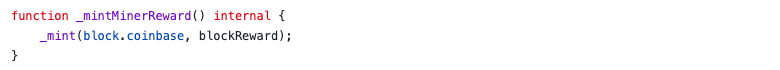
\includegraphics[scale=0.6]{IMAGES/code3.png}
        \label{fig_vsc}
    \end{figure}

    \textit{Викликає функцію з базового контракту ERC20, де параметрами є адреса майнера, який добуває поточний блок та кількість токенів, яка буде створена як винагорода для майнера. Крім цього, адреса автоматично оновлюється для кожного нового блоку, а кількість токенів встановлюється в конструкторі контракту і може бути змінена власником контракту за допомогою функції \texttt{setBlockReward}.}

    \item Внутрішня функція-захисник \texttt{\_beforeTokenTransfer}, яка викликається перед кожним переказом токенів:

    \begin{figure}[ht]
        \centering
        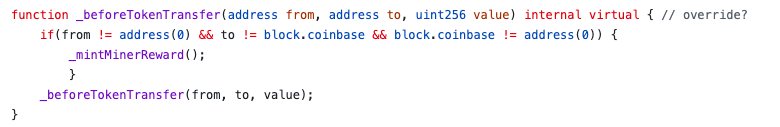
\includegraphics[scale=0.6]{IMAGES/code4.png}
        \label{fig_vsc}
    \end{figure}

    \textit{Вона додає додаткову логіку перед кожним переказом токенів. В даному випадку вона перевіряє, чи переказ токенів не відбувається з нульової адреси або до майнера, та видає винагороду за блок майнеру, якщо всі умови виконуються. Це забезпечує правильну роботу системи винагород за допомогою токенів та уникнення непотрібного видання винагороди.}
    
    \item Публічна функція \texttt{setBlockReward}, яка дозволяє власнику контракту змінювати винагороду за блок:

    \begin{figure}[ht]
        \centering
        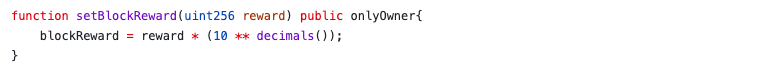
\includegraphics[scale=0.6]{IMAGES/code5.png}
        \label{fig_vsc}
    \end{figure}

    \textit{Вона забезпечує можливість динамічного налаштування винагороди відповідно до змін в мережі або економічних умов. Така гнучкість дозволяє оптимізувати роботу мережі та забезпечити адаптацію до змінних умов.}

    \newpage
    \item Публічна функція \texttt{destroy}, що дозволяє власнику контракту вивести всі ефіри з контракту та перевести їх на свій адрес:

    \begin{figure}[ht]
        \centering
        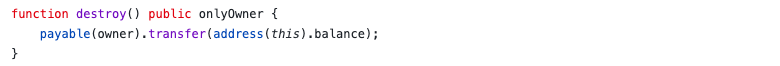
\includegraphics[scale=0.6]{IMAGES/code6.png}
        \label{fig_vsc}
    \end{figure}

    \textit{Вона забезпечує можливість закінчити дію контракту та отримати доступ до його ефірних коштів після завершення його виконання. Така можливість корисна у випадках, коли контракт вже не потрібен та його діяльність потрібно завершити.}

    \item Модифікатор \texttt{onlyOwner}, який перевіряє, чи викликаючий адрес є власником контракту:

    \begin{figure}[ht]
        \centering
        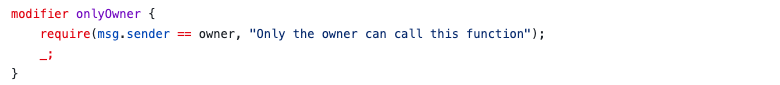
\includegraphics[scale=0.6]{IMAGES/code7.png}
        \label{fig_vsc}
    \end{figure}

    \textit{Якщо ні, генерується помилка "Тільки власник може викликати цю функцію". Даний модифікатор забезпечує безпеку, обмежуючи доступ до певних функцій лише для власника контракту. Це дозволяє захистити важливі операції від неправомірного використання та забезпечити контроль над функціоналом контракту.}
    
\end{enumerate}

\newpage

\section{Ініціалізація Hardhat}

Для початку відбувається встановлення всіх необхідних компонентів для запуску Hardhat. Для цього необхідно спочатку на ваш пристрій завантажити та встановити останньої версії такі інструменти, як npm та node.js з сайту \url{https://nodejs.org/en}. Далі встановити сам Hardhat останньої версії (опційно, окремо від плагіну в VSC) за допомогою команди в терміналі:

\begin{lstlisting}[language=bash, basicstyle=\ttfamily]
npm install --save-dev hardhat
\end{lstlisting} 

Варто зазначити, що вже після створення папки проєкту, але ще перед самим початком написання смарт-контракту, необхідно ініціалізувати проєкт hardhat за допомогою введення команди в терміналі:

\begin{lstlisting}[language=bash, basicstyle=\ttfamily]
npx hardhat init
\end{lstlisting} 

    \begin{figure}[ht]
        \centering
        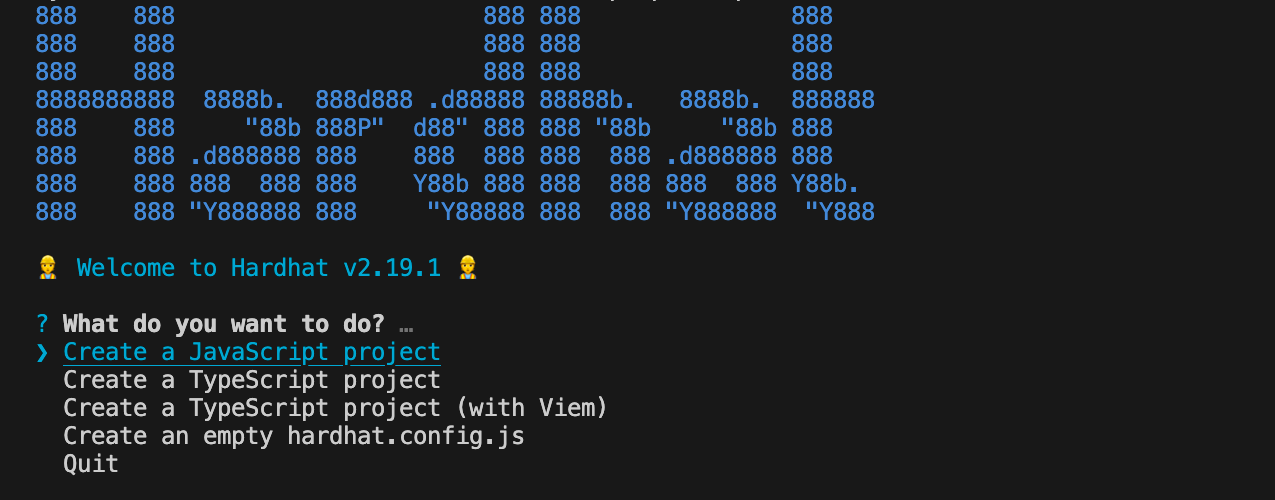
\includegraphics[scale=0.35]{IMAGES/hardhat-init.png}
        \label{fig_vsc}
    \end{figure}

Це створить вже готову структуру проєкту з необхідними нам шаблонами як основних (\texttt{deploy.js}), так і конфігураційних файлів (\texttt{hardhat.config.js}), які далі потрібно було лише відредагувати під себе.

\section {Компілювання, тестування та розгортання смарт-контракту}

Після ініціалізації Hardhat в проєкт та безпосередньо написання самого смарт-контракту, далі йде процес компілювання даного смарт-контракту та перевірки на помилки. Це відбувається за допомогою команди \texttt{npx hardhat compile} в терміналі: 

    \begin{figure}[ht]
        \centering
        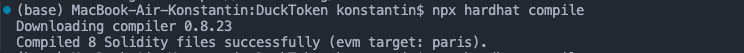
\includegraphics[scale=0.6]{IMAGES/hardhat-compile.png}
        \label{fig_vsc}
    \end{figure}


Також обов'язково перевіряємо на коректність роботи всіх функцій при симуляції всіх можливих ситуацій. Для цього необхідно написати відповідні тести в папці \texttt{test} проєкту в файлі \texttt{DuckToken.js}. А потім запустити команду \texttt{npx hardhat test} в терміналі:

    \begin{figure}[ht]
        \centering
        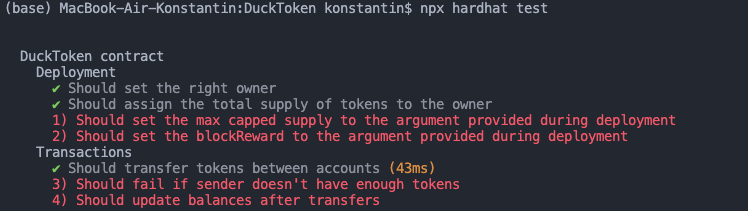
\includegraphics[scale=0.6]{IMAGES/hardhat-test.png}
        \label{fig_vsc}
    \end{figure}

Після всіх перевірок та тестувань, переходимо до найголовнішого та найважливішого етапу --- розгортання контракту або інакше -- деплой. Для цього потрібно коректно заповнити файл \texttt{deploy.js} в папці \texttt{scripts} проєкту. Після чого виконати команду в терміналі:
\begin{lstlisting}[language=bash, basicstyle=\ttfamily]
npx hardhat run scripts/deploy.js --network sepolia
\end{lstlisting} 

    \begin{figure}[ht]
        \centering
        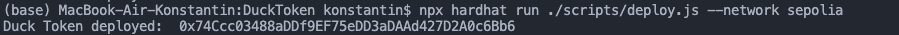
\includegraphics[scale=0.5]{IMAGES/hardhat-deploy.png}
        \label{fig_vsc}
    \end{figure}

Бачимо, що контракт нашого токену розгорнувся успішно і ми маємо адресу даного контракту в тестовій мережі Sepolia --- \href{https://sepolia.etherscan.io/address/0x74ccc03488addf9ef75edd3adaad427d2a0c6bb6}{\texttt{0x74Ccc03488aDDf9EF75eDD3aDAAd427D2A0c6Bb6}}.

Можемо перейти за посиланням в адресі та подивитися вже розгорнутий власний смарт-контракт токена:

    \begin{figure}[ht]
        \centering
        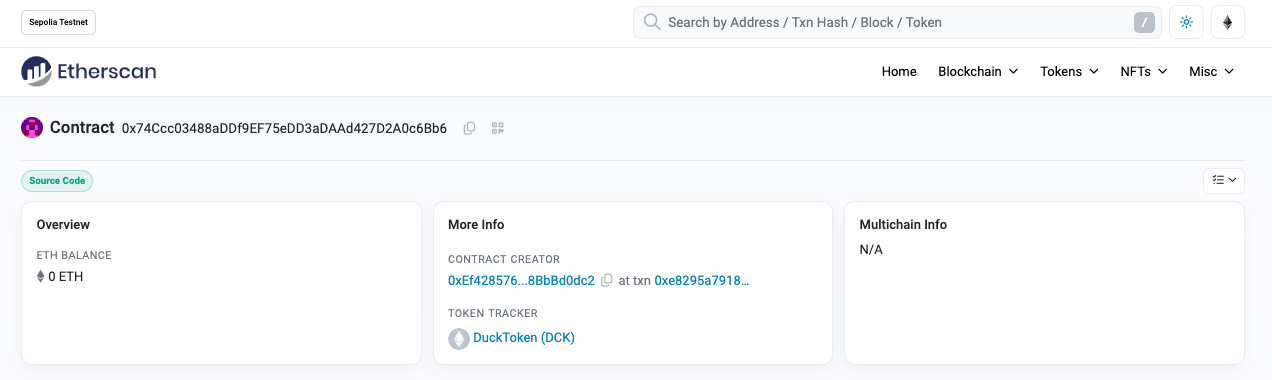
\includegraphics[scale=0.35]{IMAGES/etherscan-contract.png}
        \label{fig_vsc}
    \end{figure}

\section {Верифікація смарт-контракту}

Спочатку потрібно встановити додатковий комопонент harhdat для верифікації контрактів за допомогою команди в терміналі:
\begin{lstlisting}[language=bash, basicstyle=\ttfamily]
npx install --save-dev @nomicfoundation/hardhat-verify
\end{lstlisting} 

Після чого можемо верифікувати наш вже розгорнутий смарт-контракт токену в тестовій мережі Sepolia за допомогою команди в терміналі:

\begin{lstlisting}[language=bash, basicstyle=\ttfamily]
npx hardhat verify --network sepolia
\end{lstlisting}
\begin{lstlisting}[language=bash, basicstyle=\ttfamily]
0x74Ccc03488aDDf9EF75eDD3aDAAd427D2A0c6Bb6 "100000000" "50"
\end{lstlisting}

    \begin{figure}[ht]
        \centering
        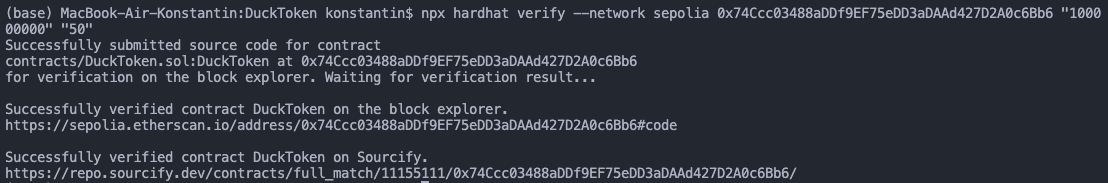
\includegraphics[scale=0.4]{IMAGES/hardhat-verify.png}
        \label{fig_vsc}
    \end{figure}

Бачимо, що операція пройшла успішно та можемо перейти за посиланням і побачити, що код нашого смарт-контракту успішно верифікований:

    \begin{figure}[ht!]
        \centering
        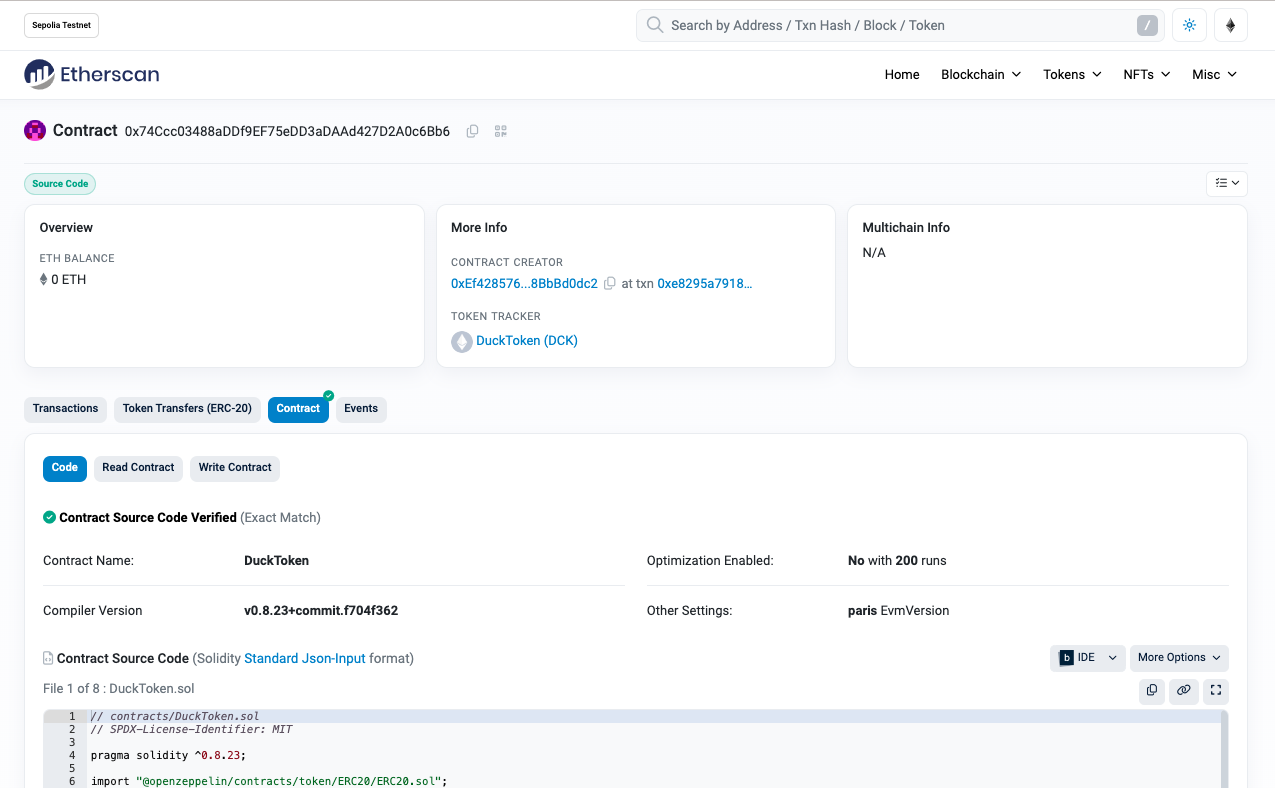
\includegraphics[scale=0.345]{IMAGES/etherscan-verify-code.png}
        \label{fig_vsc}
    \end{figure}

    \begin{figure}[ht!]
        \centering
        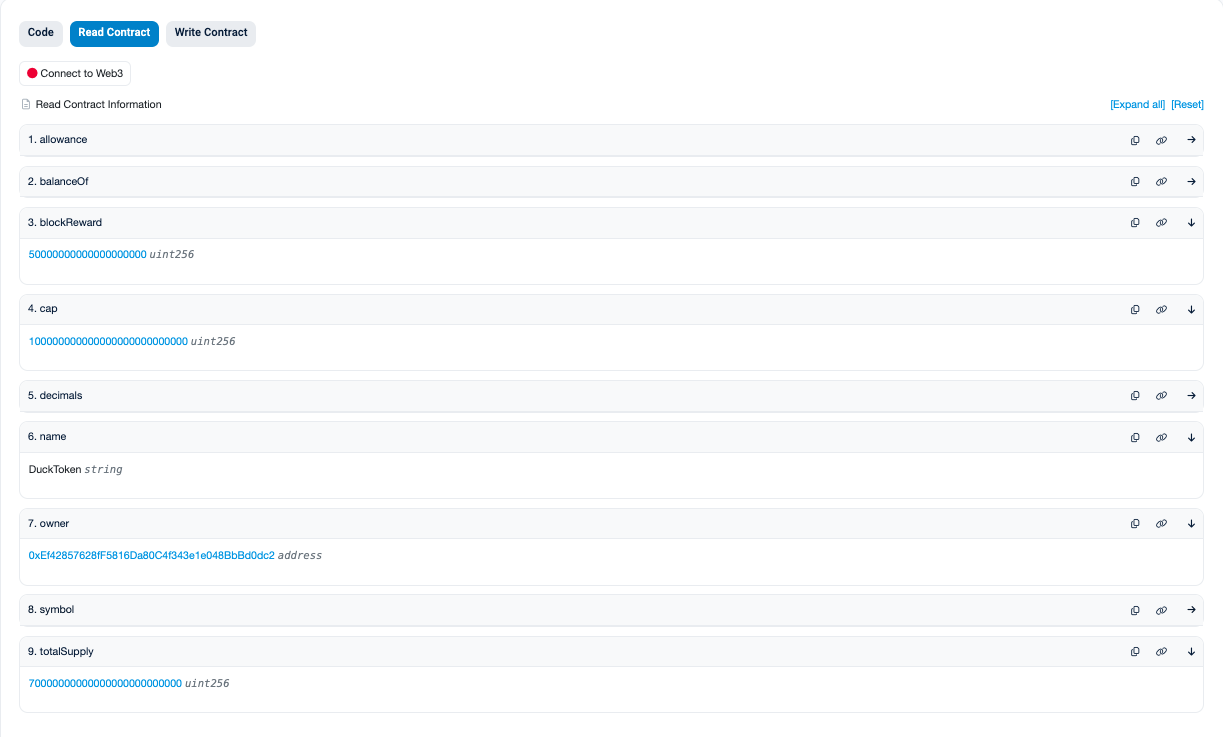
\includegraphics[scale=0.345]{IMAGES/etherscan-reading.png}
        \label{fig_vsc}
    \end{figure}

    \begin{figure}[ht!]
        \centering
        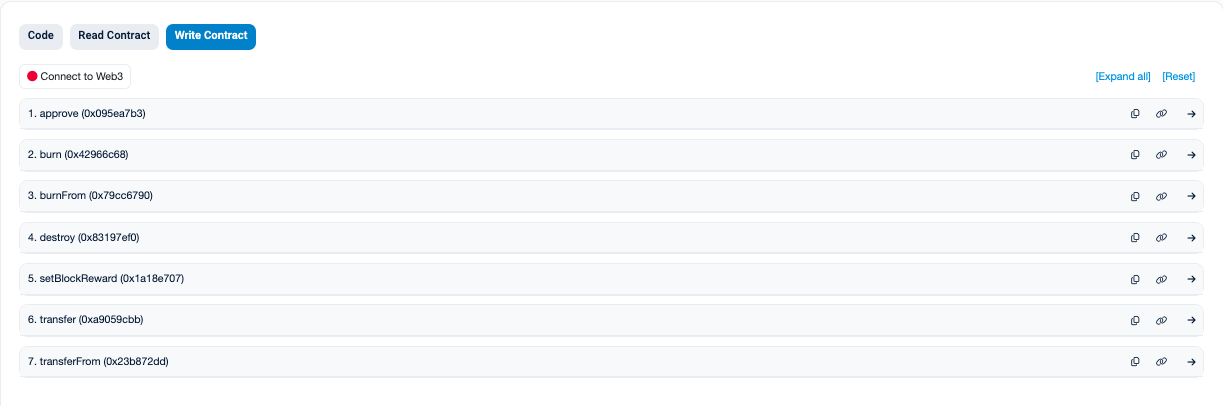
\includegraphics[scale=0.345]{IMAGES/etherscan-writing.png}
        \label{fig_vsc}
    \end{figure}

\newpage
Бачимо, що вся функціональність смарт-контракту присутня і доступна.
Крім цього, можемо перевірити функціональність та її коректність за допомогою онлайн середовища розробки смарт-контрактів в мережі Ethereum --- \href{https://remix.ethereum.org/}{Remix IDE}:

    \begin{figure}[ht]
        \centering
        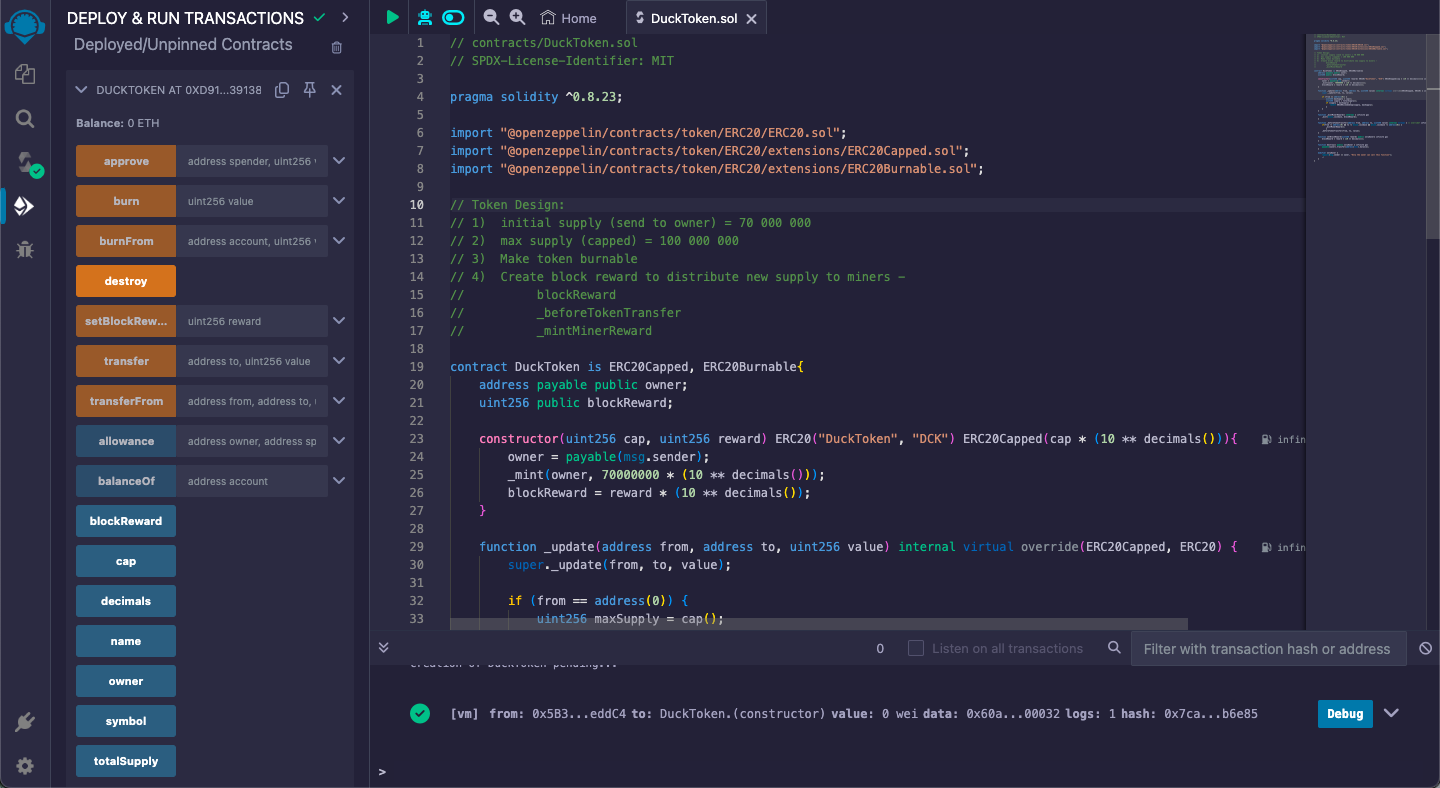
\includegraphics[scale=0.3]{IMAGES/remixIDE.png}
        \label{fig_vsc}
    \end{figure}

\section{Імпорт токенів DCK в MetaMask}

Можемо перевірити, що в нашому гаманці доступні ті 70 000 000 токенів DCK, які були прописані в смарт-контракті для власника. Для цього переходимо в наш MetaMask-гаманець та натискаємо на "Import tokens":

    \begin{figure}[ht]
        \centering
        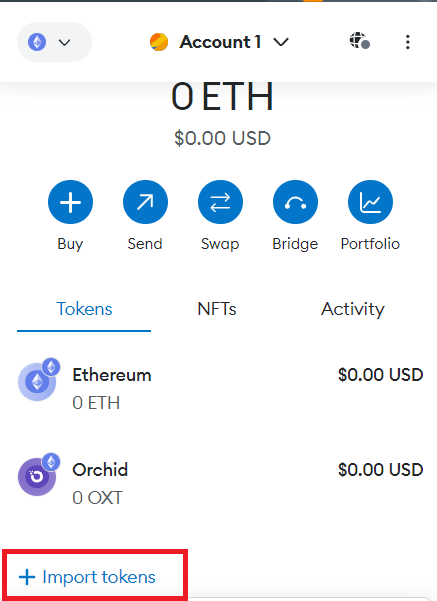
\includegraphics[scale=0.5]{IMAGES/metamask01.png}
        \label{fig_vsc}
    \end{figure}

Далі вводимо в поле адресу нашого смарт-контракту токена, після чого відбувається автоматичне заповнення інших необхідних даних, переходимо до наступного кроку -- підтверджуємо імпорт показаної нам суми токенів. В результаті отримуємо сповіщення про успішний імпорт нового токена і бачимо, що токени DCK тепер відображаються в гаманці MetaMask:

    \begin{figure}[ht!]
        \centering
        \begin{subfigure}{0.25\textwidth}
            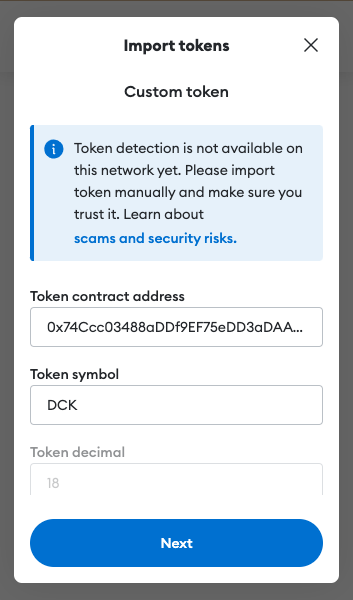
\includegraphics[width=\textwidth]{IMAGES/metamask02.png}
            \label{fig_vsc}
        \end{subfigure}
        \hfill
        \begin{subfigure}{0.25\textwidth}
             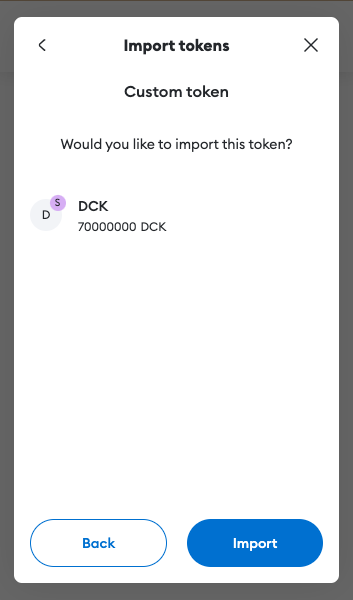
\includegraphics[width=\textwidth]{IMAGES/metamask03.png}
            \label{fig_vsc}
        \end{subfigure}
        \hfill
        \begin{subfigure}{0.25\textwidth}
             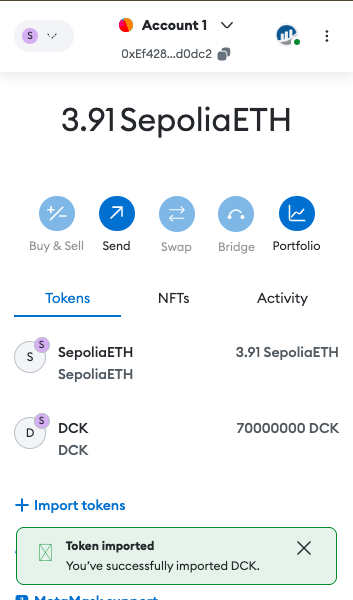
\includegraphics[width=\textwidth]{IMAGES/metamask04.png}
            \label{fig_vsc}
        \end{subfigure}
    \end{figure}

Переглянути смарт-контракт токена ERC20 --- DuckToken (DCK): \url{https://sepolia.etherscan.io/token/0x74ccc03488addf9ef75edd3adaad427d2a0c6bb6}

    \begin{figure}[ht!]
        \centering
        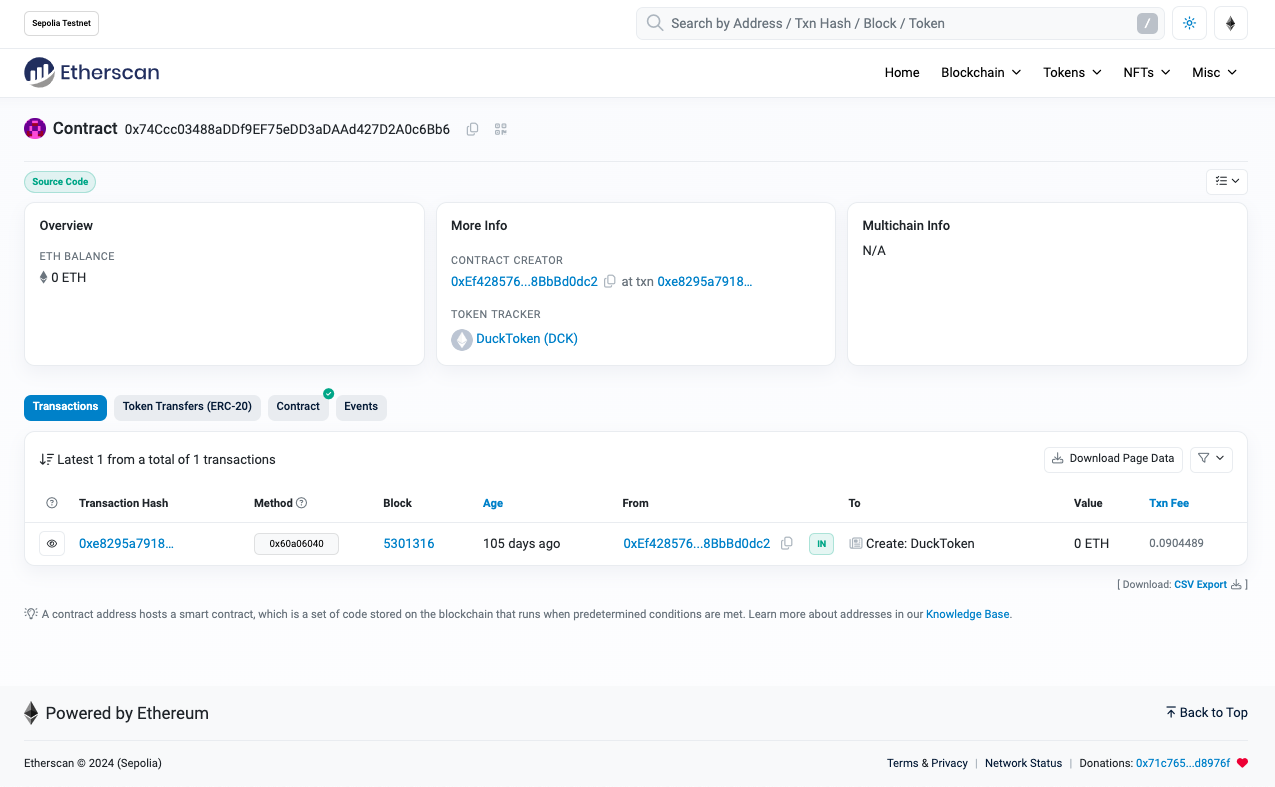
\includegraphics[scale=0.32]{IMAGES/etherscan-token.png}
        \label{fig_vsc}
    \end{figure}

% \chapconclude{\ref{chap:theory}}

% Наприкінці розділу знову наводяться коротенькі підсумки.